\fontsize{14pt}{22.5pt}\selectfont

\section{CƠ SỞ LÝ THUYẾT}
\label{ch:theory}

\indent Chương này thiết lập nền tảng lý thuyết cho toàn bộ đồ án. Trước hết, chương
điểm lại quá trình phát triển của trí tuệ nhân tạo trong game, từ các kỹ thuật lập
trình hành vi truyền thống đến sự trỗi dậy của học máy. Tiếp đó, chương trình bày các
khái niệm nền tảng của học tăng cường, bao gồm quá trình quyết định Markov, chính sách
và hàm giá trị, rồi mở rộng sang học tăng cường sâu. Phần trọng tâm của chương phân
tích nguyên lý hoạt động cùng ưu nhược điểm của ba thuật toán được sử dụng trong đề
tài, và cuối cùng giới thiệu nền tảng Unity ML-Agents cùng những giới hạn tích hợp của
nó.

\subsection{Trí tuệ nhân tạo trong game}
\indent Trí tuệ nhân tạo trong game có lịch sử phát triển song hành với sự ra đời
của ngành công nghiệp game từ những thập niên 1970-1980. Khác với AI trong nghiên
cứu học thuật, AI trong game không nhất thiết phải tối ưu hay thông minh tuyệt đối
- mục tiêu cốt lõi là tạo ra những đối thủ hoặc nhân vật phi người chơi (NPC) có
hành vi đủ thuyết phục, góp phần mang lại trải nghiệm thú vị và thử thách cho người
chơi \cite{millington2019ai}. Theo thời gian, AI trong game đã trải qua hai giai đoạn
phát triển rõ rệt: từ các kỹ thuật lập trình hành vi cứng nhắc dựa trên quy tắc đến
các phương pháp học máy có khả năng thích nghi và tự cải thiện.

\subsubsection{AI truyền thống}
\indent Trong giai đoạn đầu, AI game chủ yếu dựa trên các hệ thống quy tắc cứng
(rule-based systems), trong đó lập trình viên định nghĩa trước toàn bộ hành vi của
NPC dưới dạng tập hợp các điều kiện và phản ứng tương ứng. Cách tiếp cận này dễ
kiểm soát và dự đoán được, nhưng thiếu tính linh hoạt khi gặp các tình huống ngoài
dự kiến.

\indent Để khắc phục hạn chế đó, máy trạng thái hữu hạn (Finite State Machine -
FSM) được ứng dụng rộng rãi trong những thập niên 1990-2000. FSM mô hình hóa hành
vi của NPC thông qua một tập hữu hạn các trạng thái (tuần tra, truy đuổi, tấn công,
rút lui) và các điều kiện chuyển trạng thái tương ứng. Nhờ tính đơn giản và hiệu quả
tính toán cao, FSM vẫn được sử dụng phổ biến trong nhiều thể loại game đến tận ngày
nay \cite{millington2019ai}. Tuy nhiên, khi số lượng trạng thái và điều kiện chuyển
tiếp tăng lên, FSM nhanh chóng trở nên phức tạp và khó bảo trì, dẫn đến hiện tượng
thường được gọi là ``state explosion''.

\indent Để giải quyết bài toán lập kế hoạch hành động phức tạp hơn, Goal-Oriented
Action Planning (GOAP) được giới thiệu và phổ biến qua tựa game F.E.A.R.
(2005) \cite{millington2019ai}. Thay vì định nghĩa cứng các chuyển trạng thái, GOAP
cho phép NPC tự lập kế hoạch hành động dựa trên mục tiêu hiện tại và trạng thái thế
giới, mang lại hành vi linh hoạt và tự nhiên hơn đáng kể. Dù vậy, toàn bộ tri thức
trong GOAP vẫn phải được lập trình thủ công bởi con người, khiến chi phí xây dựng
và mở rộng hệ thống tăng cao khi độ phức tạp của game tăng lên.

\subsubsection{AI học máy}
\indent Sự bùng nổ của học máy trong thập niên 2010 đã mở ra một
hướng tiếp cận hoàn toàn mới cho AI trong game. Thay vì lập trình hành vi thủ công,
các kỹ thuật học máy cho phép agent tự học từ dữ liệu hoặc từ tương tác với môi
trường. Trong số các hướng tiếp cận đó, học tăng cường (Reinforcement Learning -
RL) nổi lên như phương pháp phù hợp nhất với bản chất của game: agent học cách hành
động thông qua thử và sai, nhận phần thưởng hoặc hình phạt từ môi trường, và dần dần
tối ưu hóa chiến lược của mình để đạt điểm số cao nhất \cite{sutton2018reinforcement}.

\indent Bước ngoặt quan trọng đến vào năm 2013 khi DeepMind công bố thuật toán
DQN (Deep Q-Network) \cite{mnih2015humanlevel}, lần đầu tiên chứng minh một agent RL
có thể học chơi thành thạo 49 trò chơi Atari khác nhau chỉ từ dữ liệu pixel thô mà
không cần bất kỳ tri thức nào được lập trình sẵn. Thành tựu này đánh dấu sự ra đời
của Deep Reinforcement Learning - kết hợp sức mạnh biểu diễn của mạng nơ-ron sâu
với khả năng học từ tương tác của RL.

\indent Những năm tiếp theo chứng kiến hàng loạt thành tựu ấn tượng: AlphaGo và
AlphaGo Zero \cite{silver2016mastering, silver2017mastering} chinh phục cờ vây ở
trình độ kiện tướng thế giới; OpenAI Five \cite{openai2019dota} đánh bại các đội
chuyên nghiệp trong Dota~2; AlphaStar \cite{vinyals2019grandmaster} đạt danh hiệu
Grandmaster trong StarCraft~II. Các kết quả này không chỉ có giá trị học thuật mà
còn mở ra tiềm năng ứng dụng RL trực tiếp trong phát triển game thương mại, từ việc
tạo NPC thông minh đến sinh nội dung tự động và hỗ trợ kiểm thử game \cite{yannakakis2018artificial}.

\subsection{Nền tảng Reinforcement Learning}

\indent Học tăng cường (Reinforcement Learning - RL) là một nhánh của học máy trong
đó một tác nhân hay còn gọi là agent học cách hành động thông qua tương tác trực tiếp với môi
trường. Khác với học có giám sát, RL không yêu cầu dữ liệu gán nhãn
sẵn có; thay vào đó, agent tự khám phá không gian hành động và nhận phản hồi dưới
dạng phần thưởng hoặc hình phạt để dần dần cải thiện chiến lược của mình
\cite{sutton2018reinforcement}. Đây là đặc tính cốt lõi khiến RL trở nên phù hợp
với các bài toán game, nơi hành vi tối ưu thường khó định nghĩa tường minh nhưng lại
dễ đánh giá thông qua kết quả.

\subsubsection{Các khái niệm cơ bản}

\indent Vòng lặp tương tác trong RL được xây dựng xung quanh năm khái niệm nền tảng.
Agent là thực thể ra quyết định - trong bối cảnh game, agent có thể là
nhân vật người chơi, NPC hay robot mô phỏng. 

\indent Environment hay môi trường là thế giới mà agent tương tác, bao gồm toàn bộ các đối tượng, luật chơi và cơ chế phản hồi; trong đề tài này, môi trường là các scene 3D được xây dựng trong Unity.

\indent State hay trạng thái $s \in \mathcal{S}$ là biểu diễn của môi trường
tại một thời điểm nhất định mà agent có thể quan sát được. Trong môi trường 3D, state
thường bao gồm vị trí, vận tốc của các đối tượng, khoảng cách đến mục tiêu và các
thông tin không gian liên quan. Action hay hành động $a \in \mathcal{A}$ là
tập hợp các lựa chọn mà agent có thể thực hiện tại mỗi bước, có thể là rời rạc như di chuyển lên,xuống,trái,phải hoặc liên tục như lực đẩy
theo trục $x$, $y$, $z$.

\indent Reward hay phần thưởng $r_t \in \mathbb{R}$ là tín hiệu phản hồi mà
môi trường trả về sau mỗi hành động của agent, đóng vai trò là thước đo duy nhất để
agent đánh giá chất lượng quyết định của mình. Việc thiết kế hàm phần thưởng hợp lý
là một trong những bước quan trọng và khó nhất trong quá trình xây dựng hệ thống RL,
vì một hàm phần thưởng không phù hợp có thể dẫn đến hành vi không mong muốn dù thuật
toán hoạt động đúng về mặt lý thuyết \cite{sutton2018reinforcement}.

\indent Tại mỗi bước thời gian $t$, agent quan sát trạng thái $s_t$, thực hiện hành
động $a_t$, nhận phần thưởng $r_t$ và chuyển sang trạng thái mới $s_{t+1}$. Vòng lặp
này lặp lại liên tục cho đến khi episode kết thúc, tức khi agent hoàn thành nhiệm vụ,
thất bại hoặc vượt quá số bước tối đa, và hình thành nên một quỹ đạo tương tác
$\tau = (s_0, a_0, r_0, s_1, a_1, r_1, \ldots)$. Toàn bộ vòng lặp tương tác giữa agent
và môi trường được minh họa trong Hình~\ref{fig:rl_loop}. Đây là sơ đồ khái quát nhất
của mọi hệ thống học tăng cường: agent quan sát trạng thái hiện tại của môi trường,
lựa chọn một hành động dựa trên chính sách của mình, và môi trường phản hồi lại bằng
một trạng thái mới cùng một phần thưởng, cứ thế lặp đi lặp lại để agent dần cải thiện
chính sách.

\begin{figure}[H]
    \centering
    \begin{tikzpicture}[node distance=2.2cm, >=latex]
        \node[draw, rounded corners, minimum width=3cm, minimum height=1.1cm,
              fill=ppocolor!15] (agent) at (0,1.6) {Agent (Tác nhân)};
        \node[draw, rounded corners, minimum width=3cm, minimum height=1.1cm,
              fill=saccolor!15] (env) at (0,-1.6) {Environment (Môi trường)};
        \draw[->, thick] (agent.east) .. controls (4.2,1.6) and (4.2,-1.6) ..
              node[right, align=left, font=\small] {Hành động $a_t$} (env.east);
        \draw[->, thick] (env.west) .. controls (-4.2,-1.6) and (-4.2,1.6) ..
              node[left, align=right, font=\small]
              {Trạng thái $s_{t+1}$\\ Phần thưởng $r_{t+1}$} (agent.west);
    \end{tikzpicture}
    \caption{Vòng lặp tương tác giữa agent và môi trường trong học tăng cường}
    \label{fig:rl_loop}
\end{figure}

\subsubsection{Markov Decision Process (MDP)}
\label{sub:mdp}

\indent Hầu hết các bài toán RL được hình thức hóa dưới dạng Quá trình Quyết định
Markov (Markov Decision Process - MDP), một khung toán học cung cấp nền tảng lý
thuyết chặt chẽ cho việc mô hình hóa bài toán ra quyết định tuần tự trong môi trường
ngẫu nhiên \cite{puterman1994markov}. Một MDP được định nghĩa bởi bộ năm thành phần
$\mathcal{M} = (\mathcal{S}, \mathcal{A}, \mathcal{P}, \mathcal{R}, \gamma)$, trong
đó $\mathcal{S}$ là không gian trạng thái, $\mathcal{A}$ là không gian hành động,
$\mathcal{P}$ là hàm chuyển trạng thái, $\mathcal{R}$ là hàm phần thưởng và $\gamma
\in [0, 1)$ là hệ số chiết khấu.

\indent Hàm chuyển trạng thái $\mathcal{P}(s' \mid s, a)$ xác định xác suất chuyển
từ trạng thái $s$ sang trạng thái $s'$ khi thực hiện hành động $a$. Tính chất Markov
- hay còn gọi là tính không nhớ - đòi hỏi rằng trạng thái tiếp theo $s_{t+1}$
chỉ phụ thuộc vào trạng thái hiện tại $s_t$ và hành động $a_t$, không phụ thuộc vào
lịch sử trước đó:

\begin{equation}
    \mathcal{P}(s_{t+1} \mid s_t, a_t, s_{t-1}, a_{t-1}, \ldots) =
    \mathcal{P}(s_{t+1} \mid s_t, a_t)
\end{equation}

\indent Giả thiết Markov này rất quan trọng vì nó đảm bảo rằng agent chỉ cần quan
sát trạng thái hiện tại để ra quyết định tối ưu, không cần lưu trữ toàn bộ lịch sử
tương tác. Trong thực tế, nhiều môi trường game thỏa mãn gần đúng tính chất này nếu
state được thiết kế đủ phong phú để mang đầy đủ thông tin cần thiết.

\indent Hệ số chiết khấu $\gamma$ xác định mức độ agent coi trọng phần thưởng tương
lai so với phần thưởng hiện tại. Khi $\gamma$ gần 1, agent có xu hướng lập kế hoạch
dài hạn; khi $\gamma$ nhỏ, agent tập trung vào phần thưởng tức thời. Tổng phần thưởng
tích lũy có chiết khấu mà agent hướng đến tối đa hóa được định nghĩa là:

\begin{equation}
    G_t = \sum_{k=0}^{\infty} \gamma^k r_{t+k+1}
\end{equation}

\subsubsection{Policy và Value Function}

\indent Policy (chính sách) $\pi$ là hàm ánh xạ từ trạng thái sang hành
động, định nghĩa chiến lược hành động của agent. Policy có thể là tất định
$\pi: \mathcal{S} \rightarrow \mathcal{A}$ hoặc ngẫu nhiên $\pi(a \mid s) =
P(A_t = a \mid S_t = s)$, cho biết xác suất chọn hành động $a$ khi ở trạng thái $s$.
Mục tiêu của RL là tìm policy tối ưu $\pi^*$ sao cho tổng phần thưởng tích lũy kỳ
vọng là lớn nhất.

\indent Value Function hay còn được gọi là hàm giá trị đo lường mức độ tốt của một trạng thái
hoặc một cặp trạng thái-hành động khi agent tuân theo một policy nhất định. Hàm giá
trị trạng thái $V^\pi(s)$ được định nghĩa là tổng phần thưởng tích lũy kỳ vọng khi
bắt đầu từ trạng thái $s$ và tuân theo policy $\pi$:

\begin{equation}
    V^\pi(s) = \mathbb{E}_\pi \left[ G_t \mid S_t = s \right]
             = \mathbb{E}_\pi \left[ \sum_{k=0}^{\infty} \gamma^k r_{t+k+1}
               \mid S_t = s \right]
\end{equation}

\indent Hàm giá trị hành động $Q^\pi(s, a)$ (hay Q-function) mở rộng khái niệm trên
bằng cách đánh giá giá trị của việc thực hiện hành động $a$ tại trạng thái $s$ rồi
sau đó tuân theo policy $\pi$:

\begin{equation}
    Q^\pi(s, a) = \mathbb{E}_\pi \left[ G_t \mid S_t = s, A_t = a \right]
\end{equation}

\indent Mối quan hệ giữa $V^\pi$ và $Q^\pi$ được thể hiện qua phương trình Bellman
\cite{bellman1957markovian}, nền tảng lý thuyết của hầu hết các thuật toán RL hiện
đại:

\begin{equation}
    V^\pi(s) = \sum_{a} \pi(a \mid s) \, Q^\pi(s, a)
\end{equation}

\indent Policy tối ưu $\pi^*$ và hàm giá trị tối ưu $V^*(s)$, $Q^*(s,a)$ thỏa mãn
phương trình tối ưu Bellman:

\begin{equation}
    Q^*(s, a) = \mathbb{E} \left[ r_{t+1} + \gamma \max_{a'} Q^*(s_{t+1}, a')
                \mid S_t = s, A_t = a \right]
\end{equation}

\indent Trong thực tế, với không gian trạng thái lớn và liên tục như các môi trường
game 3D, việc biểu diễn chính xác $V^\pi$ hay $Q^\pi$ dưới dạng bảng tra cứu là
không khả thi. Đây là động lực dẫn đến sự ra đời của Deep Reinforcement Learning,
trong đó các hàm giá trị và policy được xấp xỉ bằng mạng nơ-ron sâu, được trình bày
chi tiết trong Mục~\ref{sub:deeprl}.

\subsection{Học tăng cường sâu}
\label{sub:deeprl}
\indent Học tăng cường sâu (Deep Reinforcement Learning) là sự kết hợp giữa học tăng cường và
mạng nơ-ron sâu (deep neural network), ra đời nhằm giải quyết hạn chế cốt lõi của RL
truyền thống khi đối mặt với các bài toán có không gian trạng thái và hành động lớn,
liên tục. Thay vì lưu trữ giá trị của từng cặp trạng thái-hành động trong bảng tra
cứu, Deep RL sử dụng mạng nơ-ron để xấp xỉ các hàm giá trị hoặc policy, cho phép
tổng quát hóa sang các trạng thái chưa từng gặp trong quá trình huấn luyện
\cite{lecun2015deep}. Đây là đặc tính then chốt khiến Deep RL có thể xử lý được các
môi trường game 3D phức tạp như trong đề tài này.

\subsubsection{Vai trò của mạng Neural Network trong RL}
\indent Trong RL truyền thống, hàm giá trị $Q(s, a)$ hoặc policy $\pi(a \mid s)$
được biểu diễn dưới dạng bảng tra cứu (lookup table), đòi hỏi mỗi cặp $(s, a)$ phải
được thăm viếng đủ nhiều lần để ước lượng chính xác. Cách tiếp cận này chỉ khả thi
với không gian trạng thái hữu hạn và nhỏ. Với các môi trường game 3D, không gian
trạng thái có thể là liên tục và có số chiều rất lớn - ví dụ, vector quan sát của
agent trong môi trường Football Table bao gồm vị trí, vận tốc của bóng và các thanh
gạt trong không gian ba chiều - khiến bảng tra cứu hoàn toàn không khả thi.

\indent Mạng nơ-ron sâu giải quyết vấn đề này bằng cách đóng vai trò là bộ xấp xỉ
hàm tổng quát (universal function approximator). Thay vì lưu trữ giá trị cho từng
trạng thái, mạng học một ánh xạ tham số hóa $f_\theta: \mathcal{S} \rightarrow
\mathbb{R}$ (đối với value function) hoặc $f_\theta: \mathcal{S} \rightarrow
\Delta(\mathcal{A})$ (đối với policy), trong đó $\theta$ là tập tham số của mạng được
tối ưu hóa qua quá trình huấn luyện. Nhờ khả năng tổng quát hóa, mạng có thể ước
lượng giá trị hoặc đưa ra hành động cho các trạng thái chưa từng gặp dựa trên sự
tương đồng với các trạng thái đã học \cite{sutton2018reinforcement}.

\indent Trong thực tế, kiến trúc mạng được lựa chọn tùy theo dạng dữ liệu quan sát.
Với dữ liệu dạng vector số thực (vị trí, vận tốc, khoảng cách), mạng fully-connected
nhiều lớp (MLP) là lựa chọn phổ biến và hiệu quả. Với dữ liệu dạng ảnh hoặc dữ liệu
không gian, mạng tích chập (CNN) thường được ưu tiên. Unity ML-Agents hỗ trợ cả hai
kiến trúc này và cho phép tùy chỉnh số lớp ẩn cũng như số đơn vị trong mỗi lớp thông
qua tệp cấu hình YAML.

\subsubsection{Phân loại: Policy-Based, Value-Based, Actor-Critic}
\indent Các thuật toán Deep RL hiện đại được phân loại thành ba nhóm chính dựa trên
đối tượng mà mạng nơ-ron học để xấp xỉ, mỗi nhóm có ưu nhược điểm riêng và phù hợp
với các dạng bài toán khác nhau.

\indent Value-Based là nhóm thuật toán trong đó mạng nơ-ron học xấp xỉ hàm
giá trị $Q(s, a)$, từ đó suy ra policy tối ưu bằng cách chọn hành động có giá trị
$Q$ cao nhất. Đại diện tiêu biểu là DQN \cite{mnih2015humanlevel}. Nhóm này hoạt
động tốt với không gian hành động rời rạc nhưng gặp khó khăn với không gian hành động
liên tục do không thể tối ưu $\max_a Q(s,a)$ một cách hiệu quả khi $\mathcal{A}$ là
liên tục.

\indent Policy-Based là nhóm thuật toán trực tiếp tham số hóa và tối ưu
policy $\pi_\theta(a \mid s)$ bằng cách tính gradient của hàm mục tiêu theo tham số
$\theta$ thông qua phương pháp policy gradient \cite{williams1992simple}. Nhóm này xử
lý tốt cả không gian hành động rời rạc lẫn liên tục, nhưng thường có phương sai cao
trong ước lượng gradient, dẫn đến quá trình huấn luyện kém ổn định. PPO
\cite{schulman2017proximal} thuộc nhóm này, bổ sung thêm cơ chế clipping để giới hạn
độ lớn của mỗi bước cập nhật, giúp ổn định quá trình huấn luyện đáng kể.

\indent Actor-Critic là nhóm kết hợp ưu điểm của cả hai nhóm trên bằng cách
duy trì đồng thời hai mạng nơ-ron: mạng actor học policy $\pi_\theta(a \mid
s)$ và mạng critic học hàm giá trị $V_\phi(s)$ hoặc $Q_\phi(s,a)$. Critic
đóng vai trò đánh giá chất lượng hành động của actor, cung cấp tín hiệu học ổn định
hơn so với việc chỉ dựa vào phần thưởng thực tế \cite{mnih2016asynchronous}. SAC
\cite{haarnoja2018soft} và MA-POCA \cite{cohen2022mapoca} đều thuộc nhóm Actor-Critic,
trong đó SAC bổ sung thêm entropy regularization để khuyến khích agent khám phá, còn
MA-POCA mở rộng kiến trúc critic sang bài toán đa tác nhân với cơ chế centralized
critic cho phép mỗi agent học dựa trên thông tin toàn cục trong quá trình huấn luyện.

\indent Bảng~\ref{tab:rl_comparison} tóm tắt vị trí của ba thuật toán được sử dụng
trong đề tài theo cách phân loại trên.

\begin{table}[H]
\centering
\caption{Phân loại các thuật toán sử dụng trong đề tài}
\label{tab:rl_comparison}
\renewcommand{\arraystretch}{1.4}
\begin{tabular}{|>{\centering\arraybackslash}p{2.5cm}
                |>{\centering\arraybackslash}p{3cm}
                |>{\centering\arraybackslash}p{3cm}
                |>{\centering\arraybackslash}p{4.5cm}|}
\hline
\textbf{Thuật toán} & \textbf{Nhóm} & \textbf{On/Off-policy} & \textbf{Phù hợp với} \\
\hline
PPO      & Policy-Based      & On-policy  & Đối kháng, điều hướng \\
\hline
SAC      & Actor-Critic      & Off-policy & Hành động liên tục    \\
\hline
MA-POCA  & Actor-Critic      & On-policy  & Hợp tác đa tác nhân   \\
\hline
\end{tabular}
\end{table}

\subsection{Các thuật toán sử dụng trong đề tài}

\indent Đề tài sử dụng ba thuật toán học tăng cường đại diện cho các hướng tiếp cận
khác nhau: PPO thuộc nhóm policy-based on-policy, SAC thuộc nhóm actor-critic
off-policy và MA-POCA là thuật toán chuyên biệt cho bài toán đa tác nhân hợp tác.
Phần này trình bày nguyên lý hoạt động và đặc điểm của từng thuật toán, làm cơ sở
cho việc lựa chọn và phân tích kết quả thực nghiệm ở các chương sau.

\subsubsection{PPO (Proximal Policy Optimization)}
\label{sub:ppo}
\indent PPO (Proximal Policy Optimization) được Schulman và cộng sự đề xuất vào năm
2017 \cite{schulman2017proximal} như một cải tiến của TRPO (Trust Region Policy
Optimization) \cite{schulman2015trust} nhằm giữ lại tính ổn định trong cập nhật
policy nhưng đơn giản hơn đáng kể về mặt triển khai. PPO hiện là một trong những
thuật toán RL phổ biến nhất trong cả nghiên cứu lẫn ứng dụng thực tế, và là thuật
toán on-policy mặc định trong Unity ML-Agents.

\indent Về nguyên lý hoạt động, PPO là thuật toán on-policy, nghĩa là dữ liệu
huấn luyện được thu thập trực tiếp từ policy hiện tại và bị loại bỏ sau mỗi lần cập
nhật. Ý tưởng cốt lõi của PPO là giới hạn độ lớn thay đổi của policy trong mỗi bước
cập nhật, tránh tình trạng policy thay đổi quá đột ngột dẫn đến suy giảm hiệu năng
không thể phục hồi - một vấn đề phổ biến trong các thuật toán policy gradient đơn
giản.

\indent PPO đạt được điều này thông qua hàm mục tiêu clipped surrogate:

\begin{equation}
    L^{\text{CLIP}}(\theta) = \mathbb{E}_t \left[
        \min \left(
            r_t(\theta) \hat{A}_t,\;
            \text{clip}\!\left(r_t(\theta),\, 1-\varepsilon,\, 1+\varepsilon\right)
            \hat{A}_t
        \right)
    \right]
\end{equation}

\noindent trong đó $r_t(\theta) = \dfrac{\pi_\theta(a_t \mid s_t)}{\pi_{\theta_\text{old}}(a_t \mid s_t)}$
là tỷ lệ xác suất giữa policy mới và policy cũ, $\hat{A}_t$ là ước lượng advantage
(mức độ hành động tốt hơn hoặc kém hơn kỳ vọng trung bình) và $\varepsilon$ là siêu
tham số clipping thường được đặt trong khoảng $[0.1, 0.2]$. Toán tử $\text{clip}$
giới hạn $r_t(\theta)$ trong khoảng $[1-\varepsilon, 1+\varepsilon]$, ngăn policy mới
lệch quá xa policy cũ trong một bước cập nhật. Hàm $\min$ đảm bảo mục tiêu luôn là
cận dưới thận trọng (pessimistic lower bound) của mục tiêu không clipped.

\indent Advantage $\hat{A}_t$ thường được ước lượng bằng Generalized Advantage
Estimation (GAE):

\begin{equation}
    \hat{A}_t = \sum_{l=0}^{\infty} (\gamma\lambda)^l \delta_{t+l}, \quad
    \delta_t = r_t + \gamma V(s_{t+1}) - V(s_t)
\end{equation}

\noindent trong đó $\lambda \in [0,1]$ là tham số cân bằng giữa bias và phương sai
của ước lượng advantage, $V(s_t)$ là giá trị trạng thái được ước lượng bởi mạng
critic.

\indent Trong mỗi iteration, PPO thu thập một batch dữ liệu từ môi trường bằng policy
hiện tại, sau đó thực hiện nhiều lần cập nhật gradient trên cùng batch đó (thường từ
3 đến 10 epochs) trước khi thu thập batch mới. Nhờ cơ chế clipping, các lần cập nhật
lặp lại này không làm policy lệch quá xa điểm xuất phát, đảm bảo tính ổn định mà
không cần tính toán tốn kém như TRPO.

\indent \textbf{Ưu điểm:} PPO có tính ổn định huấn luyện cao nhờ cơ chế clipping,
dễ triển khai và tinh chỉnh tham số, hoạt động tốt trên cả không gian hành động rời
rạc lẫn liên tục. Thuật toán được tích hợp sẵn trong Unity ML-Agents với nhiều tham
số được tối ưu theo kinh nghiệm, giúp rút ngắn đáng kể thời gian thiết lập thực
nghiệm. PPO cũng dễ dàng mở rộng sang bài toán đa tác nhân thông qua cơ chế self-play
có sẵn trong ML-Agents.

\indent \textbf{Nhược điểm:} Do là thuật toán on-policy, PPO không tái sử dụng được
dữ liệu cũ, dẫn đến hiệu quả mẫu (sample efficiency) thấp hơn so với các phương pháp
off-policy. Điều này đặc biệt bất lợi trong các môi trường mà mỗi bước tương tác tốn
nhiều thời gian tính toán. Ngoài ra, PPO nhạy cảm với việc lựa chọn siêu tham số như
learning rate, số epoch và kích thước batch, đòi hỏi phải tinh chỉnh cẩn thận cho
từng bài toán cụ thể.

\subsubsection{SAC (Soft Actor-Critic)}
\indent SAC (Soft Actor-Critic) được Haarnoja và cộng sự đề xuất vào năm 2018
\cite{haarnoja2018soft, haarnoja2018softapps} như một thuật toán actor-critic
off-policy dựa trên nguyên lý maximum entropy, hướng đến giải quyết đồng thời hai
thách thức lớn của RL: hiệu quả mẫu thấp và sự nhạy cảm với siêu tham số.

\indent Điểm khác biệt cốt lõi của SAC so với các
thuật toán RL thông thường nằm ở hàm mục tiêu. Thay vì chỉ tối đa hóa tổng phần
thưởng kỳ vọng, SAC tối đa hóa đồng thời tổng phần thưởng và entropy của policy:

\begin{equation}
    J(\pi) = \mathbb{E}_{\tau \sim \pi} \left[
        \sum_{t=0}^{T} \gamma^t \Big( r(s_t, a_t) +
        \alpha \, \mathcal{H}\!\left(\pi(\cdot \mid s_t)\right) \Big)
    \right]
\end{equation}

\noindent trong đó $\mathcal{H}(\pi(\cdot \mid s_t)) = -\mathbb{E}_{a \sim \pi}
[\log \pi(a \mid s_t)]$ là entropy của policy tại trạng thái $s_t$ và $\alpha > 0$ là
hệ số nhiệt độ (temperature) cân bằng giữa phần thưởng và entropy. Entropy cao đồng
nghĩa với policy ngẫu nhiên hơn, khuyến khích agent khám phá nhiều hành động khác
nhau thay vì hội tụ sớm về một hành động tham lam.

\indent SAC duy trì ba mạng nơ-ron: mạng actor $\pi_\theta(a \mid s)$ sinh ra phân
phối xác suất trên không gian hành động, và hai mạng critic $Q_{\phi_1}(s,a)$,
$Q_{\phi_2}(s,a)$ được huấn luyện độc lập để ước lượng hàm giá trị hành động. Việc
sử dụng hai critic song song và lấy giá trị nhỏ hơn (clipped double-Q trick) giúp
giảm thiểu hiện tượng overestimation phổ biến trong các thuật toán Q-learning:

\begin{equation}
    Q_\text{target}(s_t, a_t) = r_t + \gamma \,
    \mathbb{E}_{a' \sim \pi} \!\left[
        \min_{i=1,2} Q_{\phi_i}(s_{t+1}, a') -
        \alpha \log \pi_\theta(a' \mid s_{t+1})
    \right]
\end{equation}

\indent Là thuật toán off-policy, SAC lưu trữ toàn bộ kinh nghiệm tương tác vào
replay buffer và lấy mẫu ngẫu nhiên (mini-batch) từ buffer này để cập nhật mạng,
cho phép tái sử dụng dữ liệu cũ nhiều lần và đạt hiệu quả mẫu cao hơn đáng kể so
với PPO. Hệ số nhiệt độ $\alpha$ có thể được cố định hoặc tự động điều chỉnh theo
mục tiêu entropy mong muốn $\mathcal{H}_\text{target}$, giảm thiểu nhu cầu tinh
chỉnh siêu tham số thủ công.

\indent \textbf{Ưu điểm:} SAC có hiệu quả mẫu vượt trội so với các thuật toán
on-policy nhờ replay buffer, đặc biệt phù hợp với không gian hành động liên tục -
đặc điểm quan trọng trong môi trường Football Table của đề tài. Cơ chế entropy
regularization giúp SAC tránh hội tụ sớm về cực tiểu cục bộ và duy trì khả năng
khám phá trong suốt quá trình huấn luyện. Ngoài ra, SAC ít nhạy cảm hơn với việc
lựa chọn learning rate so với PPO, mang lại tính ổn định tốt hơn trên nhiều bài toán
khác nhau \cite{haarnoja2018softapps}.

\indent \textbf{Nhược điểm:} SAC đòi hỏi bộ nhớ lớn hơn để lưu trữ replay buffer
và chi phí tính toán mỗi bước cập nhật cao hơn do phải huấn luyện đồng thời ba mạng
nơ-ron. Do là thuật toán off-policy dựa trên replay buffer, SAC không tương thích trực
tiếp với cơ chế self-play của môi trường đối kháng, vì khi đối thủ thay đổi thì các
kinh nghiệm cũ trong buffer trở nên lỗi thời và gây nhiễu cho quá trình học. Đây cũng
là một trong những giới hạn tích hợp sẵn của ML-Agents được phân tích chi tiết ở
Mục~\ref{sub:custom}.

\subsubsection{MA-POCA (Multi-Agent POsthumous Credit Assignment)}
\indent MA-POCA được Cohen và cộng sự \cite{cohen2022mapoca} đề xuất năm 2021 như
thuật toán chuyên biệt cho bài toán học tăng cường đa tác nhân hợp tác
(cooperative multi-agent), và là thuật toán đa tác nhân mặc định trong Unity
ML-Agents. MA-POCA giải quyết hai thách thức đặc thù của môi trường đa tác nhân mà
PPO hay SAC nguyên bản khó xử lý tốt: bài toán gán công lao (credit
assignment) - xác định đóng góp của từng agent vào phần thưởng chung của cả nhóm -
và bài toán tác nhân biến động (posthumous credit) - gán công lao đúng
cách cho những agent đã kết thúc hoạt động (bị loại hoặc hoàn thành nhiệm vụ) trước
khi phần thưởng nhóm được trao.

\indent Về nguyên lý hoạt động, MA-POCA mở rộng kiến trúc actor-critic theo mô hình
huấn luyện tập trung, thực thi phân tán (centralized training with
decentralized execution). Trong quá trình huấn luyện, một mạng critic tập trung
(centralized critic) được phép quan sát trạng thái và hành động của toàn bộ
các agent trong nhóm để ước lượng giá trị chung, nhờ đó đánh giá chính xác hơn đóng
góp của từng agent. Tuy nhiên, khi triển khai thực tế, mỗi agent chỉ dựa trên quan
sát cục bộ của riêng mình để ra quyết định, đảm bảo tính khả thi và khả năng mở rộng.

\indent Điểm cải tiến cốt lõi của MA-POCA nằm ở việc sử dụng cơ chế attention để xử
lý số lượng agent thay đổi động trong một episode. Thay vì cố định số lượng agent như
các phương pháp trước \cite{lowe2017multiagent, foerster2018counterfactual},
MA-POCA cho phép agent gia nhập hoặc rời khỏi
nhóm giữa chừng mà vẫn gán công lao chính xác - đặc tính rất quan trọng trong các
game hợp tác nơi agent có thể ``chết'' hoặc hoàn thành nhiệm vụ ở các thời điểm khác
nhau. Hàm giá trị nhóm được học dựa trên tổng phần thưởng nhóm (group reward) do môi
trường cung cấp thông qua cơ chế \texttt{SimpleMultiAgentGroup} của ML-Agents.

\indent Về phần cập nhật policy, MA-POCA kế thừa hàm mục tiêu clipped surrogate và cơ
chế ước lượng advantage tương tự PPO (đều là thuật toán on-policy), nhưng thay hàm
giá trị trạng thái đơn tác nhân $V(s)$ bằng hàm giá trị nhóm dựa trên baseline tập
trung, cho phép mỗi agent nhận được tín hiệu học phản ánh đúng đóng góp của mình vào
kết quả chung.

\indent \textbf{Ưu điểm:} MA-POCA được thiết kế riêng cho bài toán hợp tác đa tác
nhân, giải quyết hiệu quả vấn đề gán công lao mà PPO độc lập (mỗi agent học riêng
lẻ) thường gặp phải. Cơ chế attention giúp thuật toán linh hoạt với số lượng agent
thay đổi. Trong ML-Agents, MA-POCA tích hợp trực tiếp với cơ chế group reward, giúp
việc thiết kế môi trường hợp tác trở nên tự nhiên và trực quan.

\indent \textbf{Nhược điểm:} Là thuật toán on-policy, MA-POCA cũng chịu hạn chế về
hiệu quả mẫu tương tự PPO. Kiến trúc centralized critic làm tăng độ phức tạp tính toán
và bộ nhớ khi số lượng agent lớn. Ngoài ra, với bài toán đơn tác nhân, MA-POCA gần như
tương đương PPO nhưng phức tạp hơn không cần thiết, nên không mang lại lợi ích rõ rệt.

\subsection{Unity ML-Agents Toolkit}
\indent Unity ML-Agents Toolkit \cite{juliani2020unity} là một framework mã nguồn mở
do Unity Technologies phát triển, cho phép xây dựng môi trường game và mô phỏng 3D
làm nền tảng huấn luyện các agent thông minh bằng học tăng cường. Được giới thiệu lần
đầu vào năm 2017 và liên tục cập nhật đến nay, ML-Agents đã trở thành một trong những
nền tảng phổ biến nhất cho nghiên cứu RL trong môi trường game nhờ khả năng tích hợp
liền mạch giữa engine đồ họa Unity và hệ sinh thái Python của cộng đồng học máy.

\subsubsection{Kiến trúc tổng thể}
\label{sub:mlarch}
\indent Kiến trúc của ML-Agents được xây dựng theo mô hình client-server, trong đó
Unity Engine đóng vai trò môi trường mô phỏng và Python đóng vai trò
backend huấn luyện. Hai thành phần này giao tiếp với nhau thông qua giao
thức gRPC qua socket, cho phép chạy đồng thời nhiều instance môi trường Unity để
tăng tốc thu thập dữ liệu.

\indent Về phía Unity, thành phần trung tâm là Agent - một MonoBehaviour
được gắn vào GameObject trong scene, chịu trách nhiệm thu thập quan sát
CollectObservations, nhận hành động OnActionReceived và tính
toán phần thưởng. Mỗi Agent được liên kết với một BehaviorParameters
component định nghĩa không gian quan sát, không gian hành động và loại hành vi (học
hoặc heuristic). Academy là singleton quản lý toàn bộ vòng lặp huấn luyện,
đồng bộ hóa các bước thời gian giữa tất cả các agent trong scene và điều phối giao
tiếp với Python backend.

\indent Về phía Python, mlagents-learn là điểm vào chính của quá trình
huấn luyện, tiếp nhận tệp cấu hình YAML và khởi tạo trainer tương ứng. Các lớp
Trainer (PPOTrainer, POCATrainer) thực hiện logic huấn luyện, bao gồm thu
thập trajectory, tính toán advantage, cập nhật tham số mạng và lưu checkpoint. Thư
viện mlagents\_envs cung cấp Python API cấp thấp cho phép tương tác trực
tiếp với môi trường Unity mà không cần đi qua trainer tích hợp sẵn.

\indent Hình~\ref{fig:mlagents_architecture} minh họa kiến trúc tổng thể của hệ
thống ML-Agents và luồng dữ liệu giữa các thành phần.

\begin{figure}[H]
    \centering
    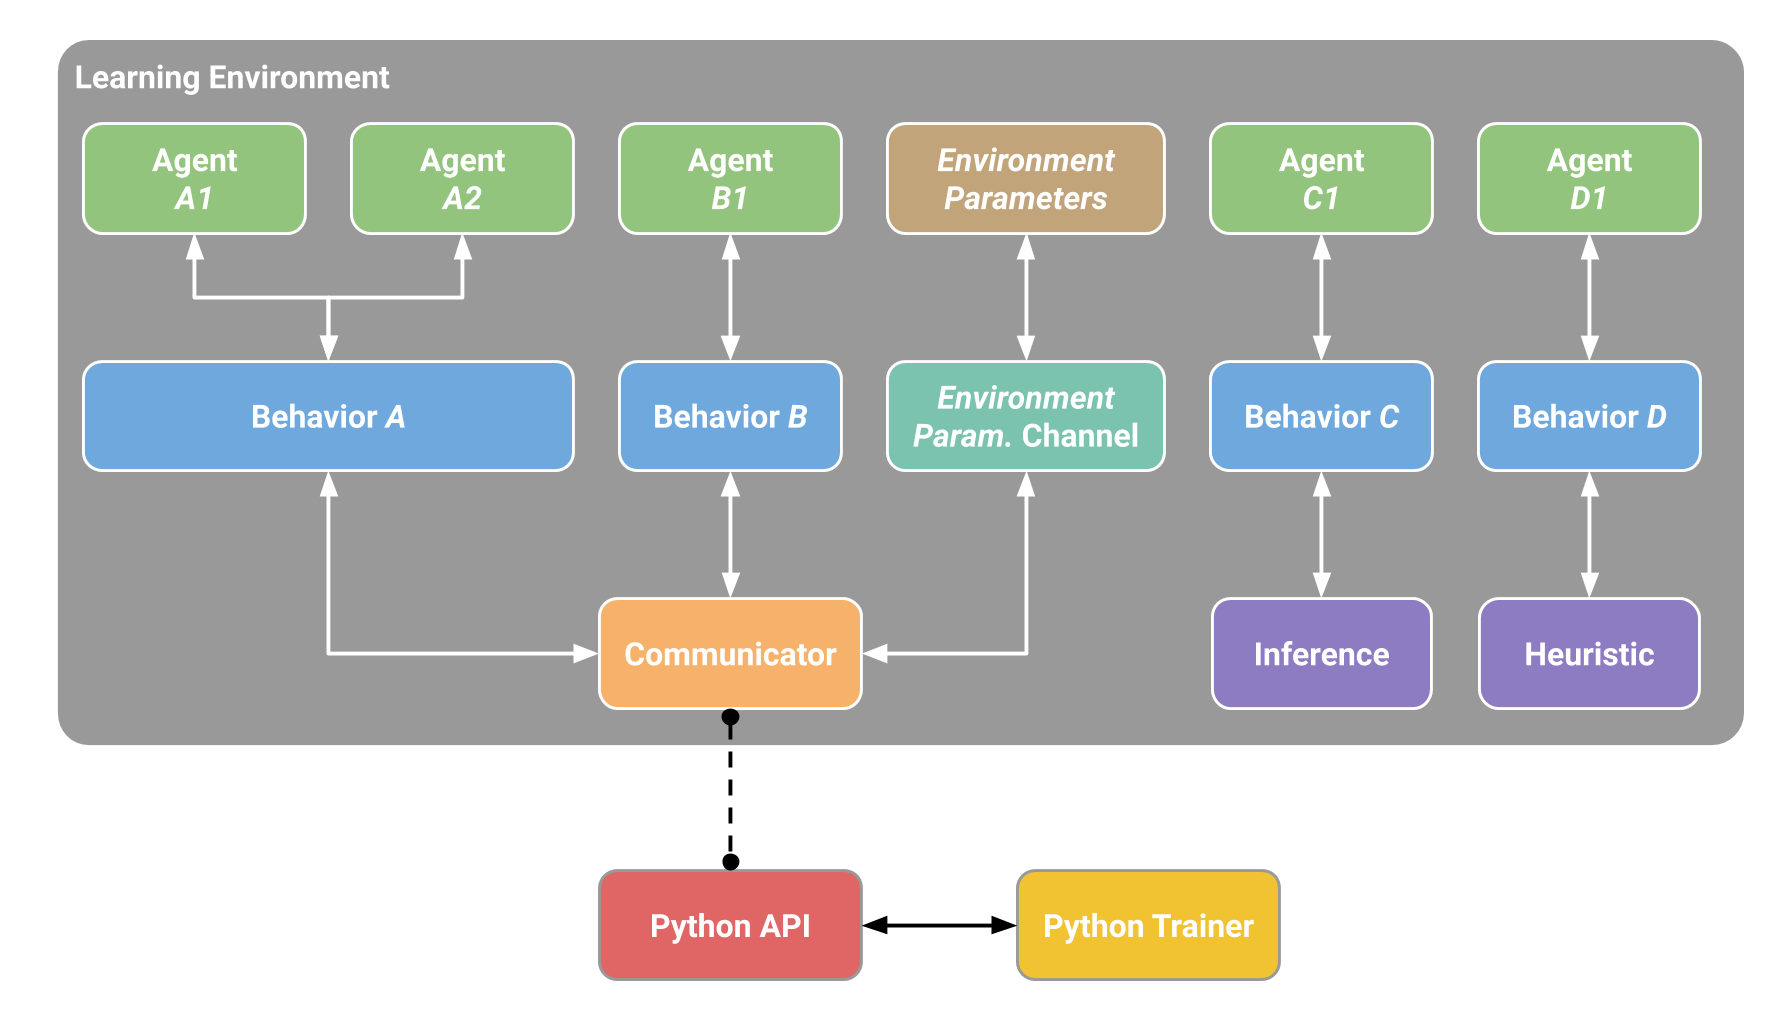
\includegraphics[width=1\textwidth]{image/learning_environment_full.png}
    \caption{Kiến trúc tổng thể của Unity ML-Agents Toolkit}
    \label{fig:mlagents_architecture}
\end{figure}

\subsubsection{Quy trình huấn luyện Agent}
\indent Quy trình huấn luyện một agent trong ML-Agents diễn ra theo vòng lặp lặp lại
liên tục cho đến khi đạt số bước tối đa hoặc người dùng dừng thủ công. Tại mỗi bước
thời gian, Unity thu thập quan sát từ tất cả các agent đang hoạt động trong scene,
gửi dữ liệu sang Python backend thông qua giao thức gRPC. Python trainer xử lý quan
sát, suy luận hành động từ policy hiện tại (hoặc lấy mẫu ngẫu nhiên trong giai đoạn
khởi động) và trả hành động về Unity. Unity thực thi hành động, cập nhật trạng thái
vật lý, tính toán phần thưởng và gửi kết quả trở lại Python để tích lũy vào buffer.

\indent Sau khi thu thập đủ một batch dữ liệu (kích thước được cấu hình qua tham số
\texttt{buffer\_size}), trainer thực hiện cập nhật tham số mạng. Đối với PPO, quá
trình cập nhật gồm nhiều epoch trên cùng batch với hàm mục tiêu clipped surrogate như
đã trình bày tại Mục~\ref{sub:ppo}. Sau khi cập nhật xong, buffer được xóa và quá trình thu
thập dữ liệu mới bắt đầu. Các chỉ số huấn luyện như cumulative reward, episode length
và policy loss được ghi lại liên tục và có thể theo dõi theo thời gian thực qua
TensorBoard.

\indent Tệp cấu hình YAML đóng vai trò trung tâm trong việc kiểm soát toàn bộ quá
trình huấn luyện. Tệp này định nghĩa loại trainer (\texttt{trainer\_type}), các siêu
tham số huấn luyện (\texttt{hyperparameters}), kiến trúc mạng nơ-ron
(\texttt{network\_settings}), cấu hình tín hiệu phần thưởng (\texttt{reward\_signals})
và số bước huấn luyện tối đa (\texttt{max\_steps}). Mỗi behavior trong scene tương
ứng với một khối cấu hình riêng, cho phép huấn luyện đồng thời nhiều loại agent với
các thiết lập khác nhau trong cùng một session. Cấu hình chi tiết cho từng thuật toán
được trình bày trong Phụ lục A, B và C.

\subsubsection{Hỗ trợ thuật toán và giới hạn tích hợp sẵn}
\label{sub:mllimits}
\indent Unity ML-Agents tích hợp sẵn hai trainer chính thức: \texttt{PPO} cho bài
toán đơn tác nhân và đối kháng (kết hợp self-play), và \texttt{POCA} (MA-POCA) cho
bài toán hợp tác đa tác nhân. Cả hai đều là thuật toán on-policy. Bên cạnh đó,
ML-Agents cũng cung cấp trainer \texttt{SAC} như một lựa chọn off-policy, cùng các
tín hiệu phần thưởng nội tại như curiosity và RND để hỗ trợ khám
phá trong môi trường phần thưởng thưa. Người dùng lựa chọn thuật toán và cấu hình siêu
tham số hoàn toàn thông qua tệp YAML mà không cần thay đổi mã nguồn C\# của môi trường.

\indent Tuy nhiên, việc tích hợp sẵn này cũng đi kèm một số giới hạn quan trọng đối
với đề tài. Thứ nhất, cơ chế self-play - vốn cần thiết cho môi trường đối
kháng như Football Table - chỉ được hỗ trợ chính thức cho PPO và POCA, mà không hỗ
trợ cho SAC. Nguyên nhân là replay buffer của SAC lưu trữ kinh nghiệm từ các phiên
bản đối thủ cũ, trở nên lỗi thời và mâu thuẫn khi đối thủ liên tục được cập nhật trong
quá trình self-play. Thứ hai, cơ chế group reward phục vụ bài toán hợp tác
được thiết kế tối ưu cho POCA; khi áp dụng cho PPO hoặc SAC, phần thưởng nhóm buộc
phải được phân bổ thủ công về từng agent, làm suy giảm khả năng gán công lao. Thứ ba,
các trainer tích hợp sẵn không cho phép người dùng dễ dàng can thiệp sâu vào vòng lặp
huấn luyện (ví dụ tùy biến hàm mất mát hay lịch trình cập nhật).

\indent Để so sánh công bằng cả ba thuật toán PPO, SAC và MA-POCA trên môi trường đối
kháng, đề tài cần một hướng tiếp cận vượt ra ngoài trainer tích hợp sẵn của ML-Agents.
Thư viện \texttt{mlagents\_envs} cung cấp Python Low-Level API cho phép điều khiển
trực tiếp môi trường Unity như một môi trường kiểu Gym, từ đó kết nối với các thư viện
RL bên ngoài như Stable-Baselines3 \cite{raffin2021stable}. Cách tiếp cận này được
trình bày chi tiết trong Mục~\ref{sub:custom}.
